\section{Data Preprocessing}

In this project, we aimed to thoroughly analyze the sentiment of textual data to gain a deeper understanding of our customers. To achieve this, we utilized three distinct datasets, each containing relevant customer feedback labeled with sentiment information. The data preprocessing steps were crucial in preparing the input for training machine learning models. Our target is to use all the models from the syllabus to accurately determine sentiment scores and uncover valuable insights into customer preferences and needs.

\subsection{Data Collection Process}

Using the datasets that we have described in the last sections, we conducted several cleaning methods for preprocessing the text to make them cleaner to some extent.\\

The datasets were sourced from Kaggle and loaded into separate pandas DataFrames.The data collection process involved downloading the datasets and loading them into our Python environment:

\begin{lstlisting}[language=Python, caption=Loading Datasets]
import pandas as pd

# Load a CSV file and initialize the Dataset class
file_path = "../../data/raw/kazanova_sentiment140_training.1600000.processed.noemoticon_with_headers.csv"
df = pd.read_csv(file_path, encoding='latin1')
dataset = Dataset(df)
file_path2 = "../../data/raw/yasserh_twitter-tweets-sentiment-dataset_Tweets_with_headers.csv"
df2 = pd.read_csv(file_path2, encoding='latin1')
dataset2 = Dataset(df2)
file_path3 = "../../data/raw/saurabhshahane_twitter-sentiment-dataset_Twitter_Data_with_headers.csv"
df3 = pd.read_csv(file_path3, encoding='latin1')
dataset3 = Dataset(df3)

# Display basic information about one of the datasets
dataset.show_overview()
\end{lstlisting}

The loaded datasets contained tweet text and sentiment labels, which were standardized before merging.

\subsection{Data Preprocessing and Merging} 

Since our project combined multiple datasets, we devised a strategy to merge them into a single cohesive dataset for analysis. The datasets had differing schemas (column names and label formats), so the first step was to standardize column names and label values across all DataFrames. We extracted the relevant columns from each DataFrame – primarily the tweet text and its sentiment label – and dropped any extraneous fields (such as tweet IDs, timestamps, or user names that were not needed for sentiment analysis). For instance, one dataset’s sentiment label was a numeric value (e.g., 0 = negative, 4 = positive), another used textual labels (“positive”, “negative”, “neutral”), and a third used -1/0/1 to denote sentiment classes. We mapped all these to a consistent labeling scheme. In our case, we unified the sentiment labels to {-1, 0, 1} representing negative, neutral, and positive sentiments respectively. For example, a tweet with label 4 (positive in the first dataset) was mapped to 1, and “negative” was mapped to -1. After aligning the schema, we merged the datasets by concatenating them vertically (appending rows) since each dataset contained unique samples. We used \texttt{pandas.concat} to combine DataFrames once their columns were made consistent. The code snippet below demonstrates how we merged DataFrames:

\begin{lstlisting}[language=Python]
from preprocess import handle_missing_values, drop_duplicates

# Standardize column names
df1.rename(columns={"target": "sentiment", "text": "text"}, inplace=True)
df2.rename(columns={"category": "sentiment", "clean_text": "text"}, inplace=True)
df3.rename(columns={"Sentiment": "sentiment", "Tweet": "text"}, inplace=True)

# Map sentiment values to a common scheme
df1["sentiment"].replace({4: 1, 0: -1}, inplace=True)
df2["sentiment"].replace({-1: -1, 0: 0, 1: 1}, inplace=True)
df3["sentiment"].replace({"Positive": 1, "Neutral": 0, "Negative": -1}, inplace=True)

# Merge datasets
combined_df = pd.concat([df1[["text", "sentiment"]], df2[["text", "sentiment"]], df3[["text", "sentiment"]]], ignore_index=True)

# Handle missing values and remove duplicates
combined_df = handle_missing_values(combined_df, strategy="mode")
combined_df = drop_duplicates(combined_df)
\end{lstlisting}

\subsection{Data Cleaning and Preparation}

After merging the datasets, we applied a series of data cleaning steps to prepare the text for analysis. We imported necessary libraries and tools for text preprocessing, including Python's \texttt{re} module for regular expressions, NLTK for tokenization and stopword lists, and custom preprocessing functions defined in our codebase. The cleaning process aimed to remove noise and standardize the text, enabling machine learning models to focus on the meaningful content of tweets. The main steps in our text cleaning pipeline were as follows:

\begin{itemize}
    \item \textbf{Removing Special Characters and Punctuation:} We filtered out all non-alphanumeric characters, such as punctuation marks and symbols (e.g., ``!!??'' or ``\ldots''), which do not carry useful sentiment information. Numerical digits (e.g., phone numbers, dates) were also removed, as they are typically uninformative for general sentiment analysis.
    
    \item \textbf{Removing URLs and HTML Tags:} Tweets often contain URLs (e.g., ``\url{http://}'' or ``\url{https://}'') or HTML markup from scraped content. Using regular expressions, we stripped substrings starting with ``http://'', ``https://'', or ``www'', as well as HTML tags (text within \texttt{< >} brackets). This ensures that only natural language content remains for sentiment analysis.

    \item \textbf{Removing Mentions and Hashtags:} We eliminated Twitter-specific artifacts like user mentions (e.g., ``@username'') and hashtags (e.g., ``\#Topic''). Mentions were removed using the regex \texttt{@\textbackslash w+}, while hashtags were handled by removing the non-alphanumeric ``\#'' symbol. This prevents the model from treating usernames or trending tags as features, as they are not generalizable signals of sentiment.

    \item \textbf{Chat Slang Expansion:} Social media text often includes slang or abbreviations (e.g., ``LOL'' for ``laugh out loud'', ``BRB'' for ``be right back''). We implemented a dictionary of common chat abbreviations, replacing them with their full meanings (e.g., ``OMG'' becomes ``oh my god''). This normalization aids sentiment analysis by converting informal terms into standard language, often preserving sentiment context (e.g., ``LOL'' may indicate humor or positivity).

    \item \textbf{Lowercasing Text:} All text was converted to lowercase to normalize words like ``Happy'' and ``happy'', reducing redundant distinctions due to capitalization. This is a standard preprocessing step to eliminate case sensitivity issues in text analysis .

    \item \textbf{Tokenization:} Each cleaned tweet was split into individual tokens (words) using NLTK's word tokenizer. For example, ``I love this movie!'' becomes \texttt{["i", "love", "this", "movie"]}. Tokenization is essential for subsequent steps like stopword removal and feature extraction.

    \item \textbf{Stopword Removal:} Common English stopwords (e.g., ``the'', ``is'', ``on'') were removed using NLTK’s built-in stopword list. These frequent words carry little sentiment value, and their removal reduces noise and data size, focusing the analysis on meaningful terms .

    \item \textbf{Stemming/Lemmatization (Optional):} Our preprocessing function included options for stemming (e.g., ``happiest'' to ``happi'') and lemmatization (e.g., ``running'' to ``run''). We primarily used lemmatization with NLTK’s WordNet lemmatizer to normalize words to their dictionary form (e.g., ``better'' to ``good''), reducing inflection variance. This step was configurable, and we analyzed results with and without it to assess its impact.
\end{itemize}

\newpage

After these steps, raw tweets were transformed into clean, standardized token sequences. For example, a tweet like:

\begin{quote}
    \small \texttt{@User OMG I love this movie!!! Check out https://t.co/xyz \#awesome}
\end{quote}

becomes:

\begin{quote}
    \small \texttt{["oh", "my", "god", "love", "movie", "awesome"]}
\end{quote}

This pipeline was applied to every tweet in the merged dataset using vectorized operations in \texttt{pandas} and \texttt{tqdm} for efficiency. The result was a new DataFrame column with cleaned text (as strings or token lists), ready for feature extraction.

\subsection{Exploratory Data Analysis (EDA)}

To better understand the dataset, we performed Exploratory Data Analysis (EDA) on key features. Below are some visualizations that provide insights into the data distribution.

\begin{figure}[H]
    \centering
    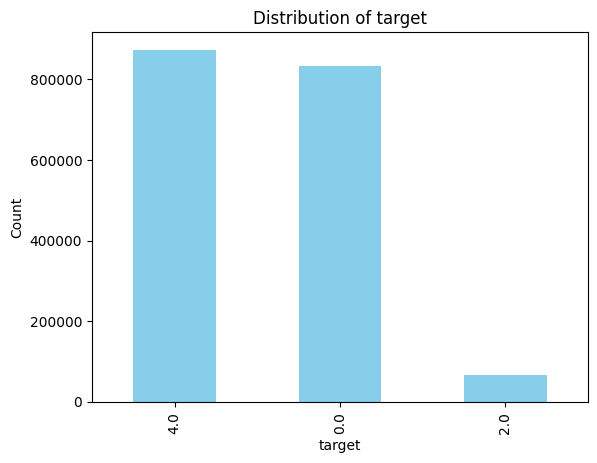
\includegraphics[width=0.7\textwidth]{img/dataset/distribution_target.png}
    \caption{Distribution of Target Variable}
    \label{fig:distribution-target}
\end{figure}

Figure~\ref{fig:distribution-target} shows the distribution of the target variable in the dataset. The dataset is imbalanced, with a significantly higher number of samples labeled as 4.0 (positive sentiment) and 0.0 (negative sentiment) compared to 2.0 (neutral sentiment). Due to this imbalance, our team decided to ignore the neutral target (2.0) and focus on training and evaluating models for positive and negative sentiment only.

\begin{figure}[H]
    \centering
    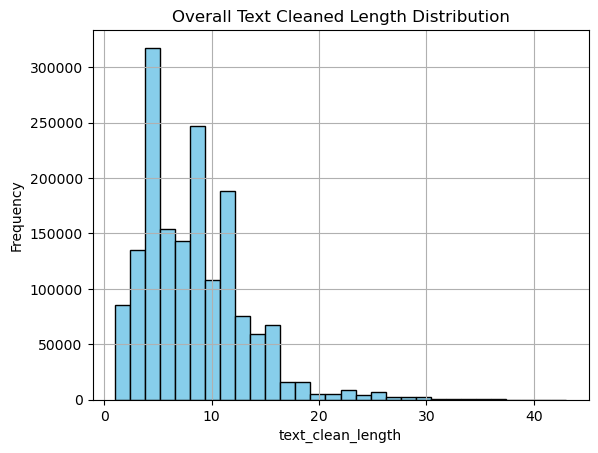
\includegraphics[width=0.7\textwidth]{img/dataset/distribution_text_clean_length.png}
    \caption{Overall Text Cleaned Length Distribution}
    \label{fig:distribution-clean-length}
\end{figure}

Figure~\ref{fig:distribution-clean-length} illustrates the distribution of cleaned text lengths across all tweets. Most tweets have a cleaned length between 5 and 15 tokens, with a long tail for shorter or longer tweets.

\begin{figure}[H]
    \centering
    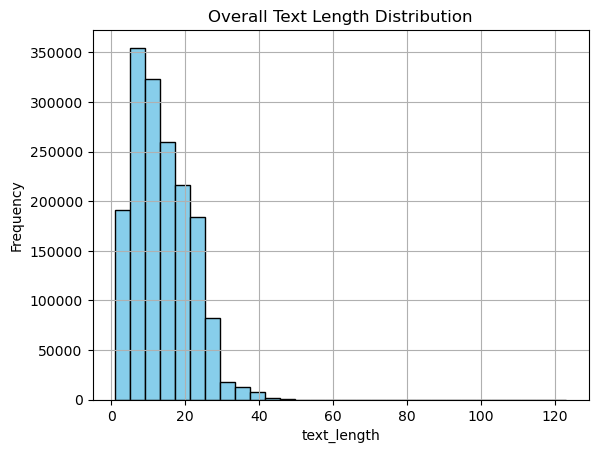
\includegraphics[width=0.7\textwidth]{img/dataset/distribution_text_length.png}
    \caption{Distribution of Raw Text Lengths}
    \label{fig:distribution-raw-length}
\end{figure}

Figure~\ref{fig:distribution-raw-length} depicts the distribution of raw text lengths before cleaning. This visualization highlights the variability in tweet lengths prior to preprocessing.

These visualizations helped us identify key patterns in the data, such as class imbalance and typical text lengths, which informed subsequent preprocessing and modeling decisions.

\subsection{Publishing the Merged Dataset on Kaggle}

We published the cleaned, merged dataset on Kaggle to enable further analysis. The process involved:

\begin{enumerate}
    \item \textbf{Saving the Dataset:} The preprocessed data was saved as \texttt{merged\_cleaned\_tweets.csv}, including cleaned text, sentiment labels, and engineered features.
    \item \textbf{Creating a New Kaggle Dataset:} On Kaggle, we created a new dataset with a descriptive title and an open license aligned with the original datasets’ terms.
    \item \textbf{Uploading the Data:} The CSV was uploaded via Kaggle’s interface or API, with column integrity verified in the preview.
    \item \textbf{Publishing:} After adding metadata (tags, visibility), the dataset was published and shared with our team for use in Kaggle Notebooks or offline analysis.
\end{enumerate}

This step ensured reproducibility and contributed a ready-to-use sentiment analysis dataset to the community. The dataset can be accessed here : \url{https://www.kaggle.com/datasets/zphudzz/tweets-clean-posneg-v1}

\subsection{Final Remarks}

The preprocessing stage laid a critical foundation for our sentiment analysis project. By merging multiple Kaggle datasets, cleaning noise (e.g., URLs, tags), and normalizing text, we enhanced data quality. Then later on, converting text to embedding vectors and encoding additional features enabled robust model training. Models trained on this preprocessed data outperformed those on raw data, highlighting the importance of these steps for accurate sentiment predictions.

\newpage
